% =====================================================================
%  Algebra 2  -  Lesson 4-3: Multiply and Divide Rational Expressions
%  Converted from Savvas enVision Algebra 2 lesson packet (DOK-labeled)
% =====================================================================
\documentclass[11pt]{article}

% ---- Packages ----
\usepackage[letterpaper,margin=0.9in,headheight=14pt]{geometry}
\usepackage{amsmath,amssymb}
\usepackage{graphicx}
\usepackage{xcolor}
\usepackage{array}
\usepackage{tabularx}
\usepackage{enumitem}
\usepackage{fancyhdr}
\usepackage{parskip}
\usepackage[most]{tcolorbox}
\usepackage{microtype}
\usepackage{hyperref}

% ---- Colors ----
\definecolor{hlcyan}{HTML}{8EF2FC}        % example-heading highlight
\definecolor{framegray}{HTML}{666666}
\definecolor{frameshade}{HTML}{F4F7FB}
\definecolor{dokred}{HTML}{B22222}
\definecolor{sentencegray}{HTML}{555555}

% ---- Fill-in blank ----
\newcommand{\blk}[1][1.2cm]{\underline{\hspace{#1}}}

% ---- Section header for Example boxes ----
\newcommand{\examplehead}[1]{%
  \vspace{6pt}%
  \noindent\colorbox{hlcyan}{\parbox{\dimexpr\linewidth-2\fboxsep}{\textbf{#1}}}%
  \vspace{2pt}%
}

% ---- DOK tag ----
\newcommand{\dok}[1]{\hfill\textit{\textbf{\textcolor{dokred}{DOK #1}}}}

% ---- Shaded sentence-frame box ----
\newtcolorbox{frames}{
  colback=frameshade, colframe=framegray!40, boxrule=0.4pt,
  arc=1pt, left=6pt, right=6pt, top=4pt, bottom=4pt,
  fontupper=\itshape\color{sentencegray}\small
}

% ---- Plain workspace box (for student written responses) ----
\newtcolorbox{workspace}[1][3]{
  colback=white, colframe=framegray!50, boxrule=0.3pt,
  arc=1pt, left=6pt, right=6pt, top=3pt, bottom=3pt,
  height=#1\baselineskip, enlarge top by=2pt, enlarge bottom by=2pt,
  valign=top
}

% ---- Turn-and-talk bullet ----
\newcommand{\turnandtalk}[1]{%
  \vspace{3pt}%
  \noindent\textbullet~\textbf{Turn and Talk:} #1\par%
}

% ---- Short-write bullet ----
\newcommand{\shortwrite}[1]{%
  \vspace{3pt}%
  \noindent\ding{97}~\textbf{Short Write:} #1\par%
}
\usepackage{pifont}   % for \ding

% ---- Running header ----
\pagestyle{fancy}
\fancyhf{}
\lhead{\small Algebra 2 -- Block \blk[0.9cm]\quad Date \blk[1.6cm]\quad Name \blk[4.2cm]}
\rhead{\small\thepage}
\renewcommand{\headrulewidth}{0pt}

% ---- Tighter spacing around display math in this packet ----
\setlength{\abovedisplayskip}{4pt}
\setlength{\belowdisplayskip}{6pt}
\setlength{\abovedisplayshortskip}{2pt}
\setlength{\belowdisplayshortskip}{4pt}

\begin{document}

% =====================================================================
% TITLE + OBJECTIVES
% =====================================================================
\begin{center}
  {\LARGE\textbf{Lesson 4-3: Multiply and Divide Rational Expressions}}
\end{center}

\noindent
\renewcommand{\arraystretch}{1.25}
\begin{tabularx}{\linewidth}{|>{\raggedright\arraybackslash}p{2.8cm}|X|}
  \hline
  \textbf{Math Objective} &
    Use structure of rational expressions to rewrite them in different forms.
    Understand that rational expressions are analogous to rational numbers
    and follow similar rules when multiplying and dividing. \\ \hline
  \textbf{Language Objective} &
    Students will explain how to state the domain of a simplified rational
    expression using sentence frames. \\ \hline
  \textbf{Essential Understanding} &
    I can find the product and the quotient of rational expressions. \\ \hline
\end{tabularx}
\renewcommand{\arraystretch}{1.0}

% =====================================================================
% 1. QUICK CHECK
% =====================================================================
\section*{1.\; Quick Check}
\noindent
\begin{tabularx}{\linewidth}{|>{\centering\arraybackslash}p{4.2cm}|X|}
  \hline
  \vspace{1pt}
  \textbf{Look at the expression:}\par
  \vspace{4pt}
  $\displaystyle \frac{x-2}{x-2}$
  \vspace{4pt}
  &
  Do you think it always equals 1?  Circle one: \par
  \vspace{6pt}
  \hfill {\large\textbf{Yes}}\hfill {\large\textbf{No}}\hfill {\large\textbf{Not sure}}\hfill\mbox{}\\ \hline
\end{tabularx}

% =====================================================================
% 2. TEST IT  |  3. EXPLAIN WHAT YOU SEE
% =====================================================================
\vspace{8pt}
\noindent
\begin{minipage}[t]{0.38\linewidth}
  \textbf{2.\; Test It}\par\vspace{4pt}
  \renewcommand{\arraystretch}{1.35}
  \begin{tabular}{|>{\centering\arraybackslash}p{1.2cm}|>{\centering\arraybackslash}p{3.0cm}|}
    \hline
    \textbf{\textit{x}} & $\displaystyle \frac{x-2}{x-2}$ \\ \hline
    0 & \\ \hline
    1 & \\ \hline
    2 & \\ \hline
    3 & \\ \hline
    4 & \\ \hline
  \end{tabular}
\end{minipage}%
\hfill
\begin{minipage}[t]{0.58\linewidth}
  \textbf{3.\; Explain What You See}\par\vspace{4pt}
  \begin{workspace}[3]\end{workspace}
  \vspace{6pt}
  \begin{frames}
    The expression \textbf{breaks} at \blk\ because dividing by zero is not allowed.\par
    It equals $1$ for all values \textbf{except} \blk\ because the denominator becomes zero.
  \end{frames}
\end{minipage}

\vspace{8pt}
\noindent Some values make an expression ``break.''  Now we will practice
rewriting expressions and checking which values are allowed.

% =====================================================================
% EXAMPLE 1
% =====================================================================
\examplehead{EXAMPLE 1 -- Write Equivalent Rational Expressions}

\noindent We can rewrite an expression by multiplying by a form of 1.

\noindent A \emph{form of 1} looks like this:
\[
  \frac{x}{x}\qquad\qquad \frac{x+2}{x+2}\qquad\qquad \frac{5}{5}
\]

\noindent These fractions all equal 1 (as long as the denominator is not zero).

\noindent\textbf{Start with the expression:}
\[ x+3 \]

\noindent\textbf{Multiply by a form of 1:}
\[ (x+3)\cdot\frac{x}{x} \]

\noindent\textbf{Rewrite it as a rational expression:}
\[ \frac{x(x+3)}{x} \]

\noindent These two expressions look different, but they represent the same
value for all $x$ except $0$.
\begin{itemize}[leftmargin=1.5em,itemsep=1pt,topsep=2pt]
  \item The original expression $x+3$ is defined for every real number.
  \item The rewritten expression $\dfrac{x(x+3)}{x}$ is undefined when $x=0$
        because the denominator becomes zero.
\end{itemize}

\noindent\textbf{So the expressions are equivalent only on the shared domain.}

\turnandtalk{Why can multiplying by 1 change the domain?}

\begin{frames}
  \textbf{Word bank:}\quad value\quad|\quad zero\quad|\quad denominator\quad|\quad restriction
\end{frames}

% -------- TRY IT 1 --------
\subsection*{TRY IT 1}
\noindent Rewrite the expression below by multiplying by a form of 1.
Then state the value that must be excluded from the domain.
\[
  x-5 \;\longrightarrow\; (x-5)\cdot\frac{x+2}{x+2}
\]

\noindent\textbf{Domain restriction:}\;\blk[4cm]

% =====================================================================
% EXAMPLE 2
% =====================================================================
\examplehead{EXAMPLE 2 -- Simplifying a Rational Expression}

\noindent A rational expression is in \textbf{simplest form} when the
numerator and denominator have \textbf{no common factors} (other than 1).

\noindent We can simplify by \textbf{canceling common factors}, but we must
also state the \textbf{domain} (values that make the denominator zero).

\noindent\textbf{Simplify the expression:}
\[
  \frac{(x-2)(x+5)}{(x-2)(x-3)}
\]

\noindent\textbf{Step 1:\; Identify the common factor}\par
Both numerator and denominator contain the factor $(x-2)$.

\noindent\textbf{Step 2:\; Cancel the common factor}
\[
  \frac{\boxed{(x-2)}\,(x+5)}{\boxed{(x-2)}\,(x-3)} \;=\; \frac{x+5}{x-3}
\]

\noindent\textbf{Step 3:\; State the domain}\par
The original denominator was $(x-2)(x-3)$.  So the expression is undefined when:
\begin{itemize}[leftmargin=1.5em,itemsep=1pt,topsep=2pt]
  \item $x = 2$
  \item $x = 3$
\end{itemize}

\noindent\textbf{Final Answer}
\[
  \frac{x+5}{x-3},\quad \text{for } x\neq 2,\;3
\]

\shortwrite{Explain why we must use the \textbf{original} denominator
(not the simplified one) to determine the domain of a rational expression.}

\begin{workspace}[3]\end{workspace}

\vspace{4pt}
\begin{frames}
\begin{tabularx}{\linewidth}{XX}
  We use the original denominator because \blk[2.5cm]\,.\; &
  Even though the factor was canceled, it still affects the domain since \blk[2.5cm]\,.\; \\
  \vspace{4pt}\par
  The simplified expression does not show the restriction at \blk\ because \blk[2.5cm]\,.\; &
  \vspace{4pt}\par
  This shows that simplifying does not change \blk[2.5cm]\,.\; \\
\end{tabularx}
\end{frames}

% -------- Try It 2 --------
\subsection*{Try It 2}
\noindent Simplify the expression and state the domain:
\[
  \frac{(y+4)(y-1)}{(y-1)(y-6)}
\]

\noindent\textbf{Simplified form:}\; \blk[5cm]
\hfill\textbf{Domain:}\; $y\neq \blk[0.6cm]$,\; $y\neq \blk[0.6cm]$

% =====================================================================
% EXAMPLE 3
% =====================================================================
\examplehead{EXAMPLE 3 -- Multiplying Rational Expressions}

\noindent When we multiply rational expressions, we multiply
\textbf{straight across} (numerator $\times$ numerator, denominator
$\times$ denominator).  Then we \textbf{cancel any common factors}.

\noindent This works exactly like multiplying numerical fractions.

\noindent\textbf{Multiply and simplify:}
\[
  \frac{x}{x+3}\;\cdot\;\frac{x+3}{x-1}
\]

\noindent\textbf{Step 1:\; Multiply across}
\[
  \frac{x(x+3)}{(x+3)(x-1)}
\]

\noindent\textbf{Step 2:\; Cancel the common factor}
\[
  \frac{\boxed{(x+3)}\cdot x}{\boxed{(x+3)}(x-1)} \;=\; \frac{x}{x-1}
\]

\noindent\textbf{Step 3:\; State the domain}\par
The original denominators were $x+3$ and $x-1$.  So the expression is
undefined when:
\begin{itemize}[leftmargin=1.5em,itemsep=1pt,topsep=2pt]
  \item $x = -3$
  \item $x = 1$
\end{itemize}

\noindent\textbf{Final Answer}
\[
  \frac{x}{x-1},\quad \text{for } x\neq -3,\;1
\]

\turnandtalk{Did canceling remove the domain restriction?  Why or why not?}

\begin{frames}
  \textbf{Word bank:}\quad cancel\quad|\quad denominator\quad|\quad restriction\quad|\quad factor\quad|\quad zero\quad|\quad original expressions
\end{frames}

% -------- Try It 3 --------
\subsection*{Try It 3}
\noindent Multiply and simplify.  Then state the domain.
\[
  \frac{x-4}{x+2}\;\cdot\;\frac{(x+2)(x+5)}{(x-4)(x-1)}
\]

\noindent\textbf{Simplified form:}\; \blk[5cm]
\hfill\textbf{Domain:}\; $x\neq \blk[0.6cm]$,\; $x\neq \blk[0.6cm]$,\; $x\neq \blk[0.6cm]$

% =====================================================================
% EXAMPLE 5
% =====================================================================
\examplehead{EXAMPLE 5 -- Dividing Rational Expressions}

\noindent To divide rational expressions, we \textbf{multiply by the
reciprocal} of the divisor.  Then we cancel any common factors and state
the domain.

\noindent\textbf{Divide and simplify:}
\[
  \frac{(x+1)(x+4)}{x-2}\;\div\;\frac{x+1}{(x-2)(x+5)}
\]

\noindent\textbf{Step 1:\; Multiply by the reciprocal}
\[
  \frac{(x+1)(x+4)}{x-2}\;\cdot\;\frac{(x-2)(x+5)}{x+1}
\]

\noindent\textbf{Step 2:\; Cancel common factors}\par
Cancel $(x+1)$ and $(x-2)$:
\[
  \frac{\boxed{(x+1)}\,(x+4)}{\boxed{(x-2)}} \;\cdot\;
  \frac{\boxed{(x-2)}\,(x+5)}{\boxed{(x+1)}}
\]

\noindent What remains:
\[
  (x+4)(x+5)
\]

\noindent\textbf{Step 3:\; State the domain}\par
The original denominators were:
\begin{itemize}[leftmargin=1.5em,itemsep=1pt,topsep=2pt]
  \item $x-2$
  \item $(x-2)(x+5)$
\end{itemize}
So the expression is undefined when:
\begin{itemize}[leftmargin=1.5em,itemsep=1pt,topsep=2pt]
  \item $x = 2$
  \item $x = -5$
  \item $x = -1$\; (from the canceled $(x+1)$ in the divisor)
\end{itemize}

\noindent\textbf{Final Answer}
\[
  (x+4)(x+5),\quad \text{for } x\neq -5,\;-1,\;2
\]

\shortwrite{Explain why dividing rational expressions can create multiple
domain restrictions, including some that come from factors that get canceled.}

\begin{workspace}[3]\end{workspace}

\vspace{4pt}
\begin{frames}
\begin{tabularx}{\linewidth}{XX}
  Division creates more restrictions because \blk[2.5cm]\,.\; &
  Even canceled factors matter because they were originally in a \blk[2.5cm]\,.\; \\
  \vspace{4pt}\par
  Any factor in the original denominators causes a restriction when \blk[2.5cm]\,.\; &
  \vspace{4pt}\par
  This means the final domain must include restrictions from \blk[2.5cm]\,.\; \\
\end{tabularx}
\end{frames}

% -------- Try It 5 --------
\subsection*{Try It 5}
\noindent\textbf{Divide and simplify.  Then state the domain.}
\[
  \frac{(x-3)(x+2)}{x+4}\;\div\;\frac{x-3}{(x+4)(x-1)}
\]

\noindent\textbf{Simplified form:}\; \blk[5cm]
\hfill\textbf{Domain:}\; $x\neq \blk[0.6cm]$,\; $x\neq \blk[0.6cm]$,\; $x\neq \blk[0.6cm]$

% =====================================================================
% REFERENCE IMAGES (Concept Summary & Fraction Rules)
% =====================================================================
\vspace{10pt}
\noindent
\begin{minipage}[t]{0.56\linewidth}
  \centering
  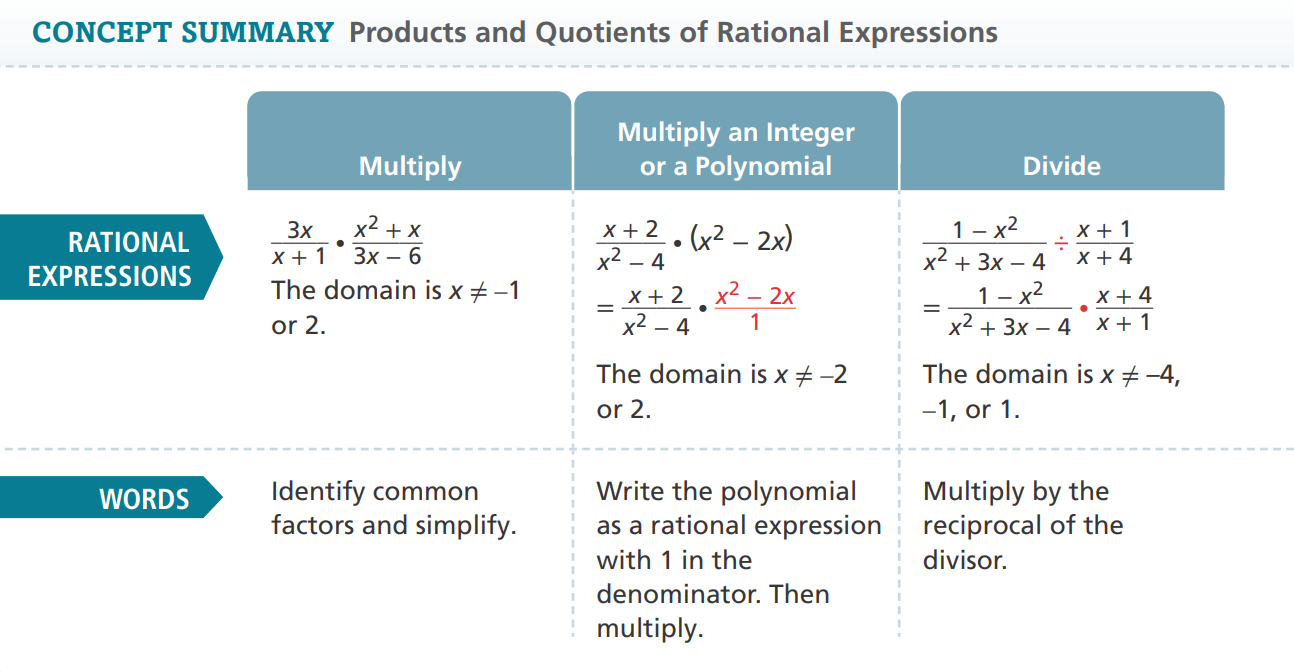
\includegraphics[width=\linewidth]{concept-summary.png}
\end{minipage}%
\hfill
\begin{minipage}[t]{0.40\linewidth}
  \centering
  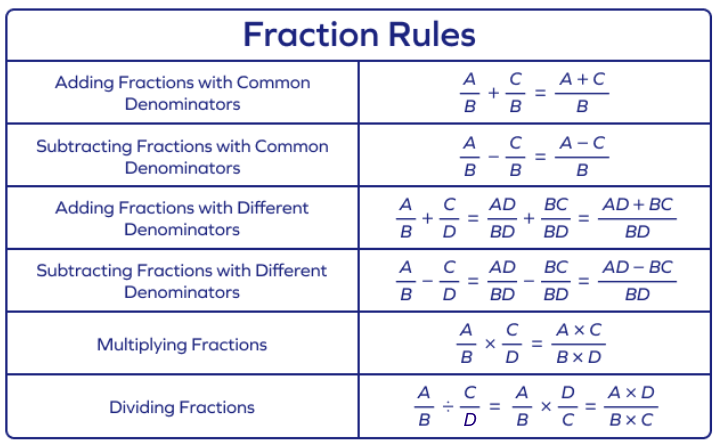
\includegraphics[width=\linewidth]{fraction-rules.png}
\end{minipage}

% =====================================================================
% SELECT EXERCISES
% =====================================================================
\begin{center}\textbf{\Large Select Exercises}\end{center}

% ---- Row 1: Error Analysis (DOK2) ----
\noindent
\begin{tabularx}{\linewidth}{|>{\raggedright\arraybackslash}p{7.8cm}|X|}
  \hline
  \vspace{2pt}
  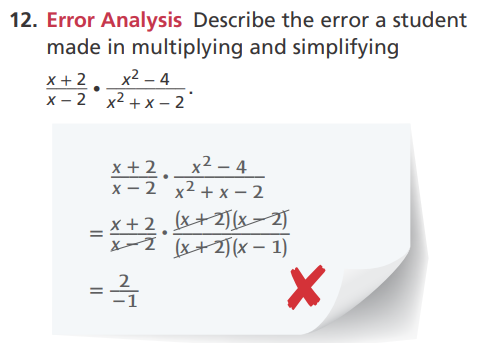
\includegraphics[width=7.3cm]{error-analysis.png}\par
  \dok{2}
  &
  \vspace{4cm}
  \\ \hline

  % ---- Row 2: Simplify (DOK1) ----
  \vspace{2pt}
  \textbf{Simplify the expression and state the domain.}\par
  \vspace{4pt}
  $\displaystyle \frac{(x-4)(x+7)}{(x-4)(x-1)}$\par
  \vspace{6pt}
  \dok{1}
  &
  \vspace{3.5cm}
  \\ \hline

  % ---- Row 3: Multiply (DOK1) ----
  \vspace{2pt}
  \textbf{Multiply, simplify, and state the domain.}\par
  \vspace{4pt}
  $\displaystyle \frac{x+3}{(x-2)(x+5)}\;\cdot\;\frac{(x-2)(x-1)}{x+3}$\par
  \vspace{6pt}
  \dok{1}
  &
  \vspace{3.5cm}
  \\ \hline

  % ---- Row 4: Divide (DOK1) ----
  \vspace{2pt}
  \textbf{Divide, simplify, and state the domain.}\par
  \vspace{4pt}
  $\displaystyle \frac{(x-6)(x+2)}{x+4}\;\div\;\frac{x-6}{(x+4)(x-3)}$\par
  \vspace{6pt}
  \dok{1}
  &
  \vspace{3.5cm}
  \\ \hline

  % ---- Row 5: Lupe carnival (DOK3) ----
  \vspace{2pt}
  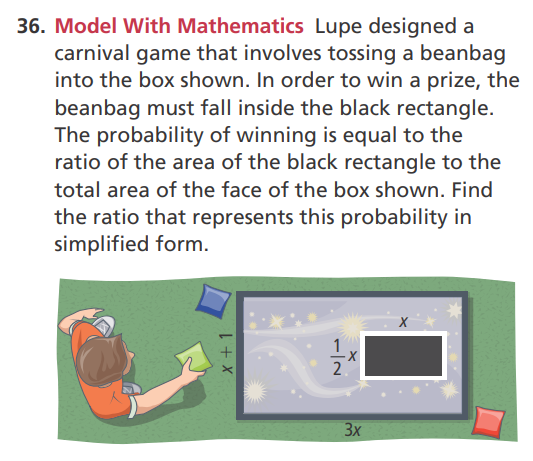
\includegraphics[width=7.3cm]{lupe-carnival.png}\par
  \dok{3}
  &
  \vspace{5cm}
  \\ \hline
\end{tabularx}

\end{document}
